\documentclass[twocolumn]{revtex4}
\usepackage{graphics,graphicx,epsfig,ulem} 
\usepackage{amsmath}
\usepackage{multirow}
\usepackage{gensymb}
\usepackage{commath}
\usepackage{textcomp}
\newcommand{\squeezeup}{\vspace{-2.5mm}}

\begin{document}

\textheight=26.385cm
%Change textheight as the last resort...

\title{Determining the viscosity of water} 
 
 
\author{Jacky Cao, Room 205, Thursday, Lab Partners: Peter Dorey, Jon Pritchett \\ Date of experiment: 11/11/2016, Date of report: 20/11/2016}


\begin{abstract}              
 
asdkjasnkdnasd

\end{abstract}

\maketitle

\section{Introduction} 
\vspace{-2ex} 

Derived experimentally by Poiseuille in 1838 and Hagen in 1839 \cite{poiseuillehagen}, the volume flow rate $dV/dt$ of a fluid passing through a tube can be expressed as a function of the density of the fluid $\rho$, the value for acceleration due to gravity $g$, the height the fluid leaves the tube $h$, the radius $a$ and length $L$ of the tube, and the viscosity of the fluid $\eta$,

\begin{equation} 
\frac{dV}{dt}=\frac{\pi}{8}\frac{\rho gh}{\eta}\frac{a^4}{L}. 
\label{pohagen}
\end{equation}

Noting that the group $\rho gh$ can be collectively termed the pressure difference $\Delta P$ between the two ends of the tube \cite{collegephysics}. [[?? add something more to here]]

If we consider that a fluid is flowing through said [[?]] tube, it experiences both friction with the inner wall and internal friction within itself. The latter can be defined more readily as the viscosity of the fluid $\eta$, and this results in shear stress when two adjacent layers (laminas) of fluid move relative to each other. 

We find that as $\eta$ increases, the volume flow rate decreases, the shear stress between two laminas becomes greater and so restricts the movement of the fluid's molecules trying to flow through the tube. 

Generally we can say that the lamina flow streamlines are smooth, top layers sliding over other laminas without the system having any turbulent motion - this condition is required for equation [\ref{pohagen}] to be valid. 

Using a rearranged form of the relation derived by Hagen and Poiseuille it is possible to experimentally calculate a value for the viscosity of water.

\vspace{-3ex}
\section{Method} 
\vspace{-2ex}
A flow of water was created by fixing a capillary tube to a water tank. The tank was raised to an initial height arbitrary height above the work surface[?]. The tank was then filled up with water from heights 2cm to 16cm at 2cm intervals, these values were measured with the markings on the side of the tank. During this we had to ensure that we did not create parallax between the level of the water and the markings on the side. 

The water was then allowed to flow out of the tube for a period of 90s for each height of water, this time was measured using a digital stopwatch. As the water flowed out it was caught within a large beaker so that the mass and volume of it could be measured after the allotted time had passed. 

The mass was found by having the beaker already on a set of electronic scales and initially zeroed to account for the beaker's mass. The volume on the other hand required the water to be transferred from the beaker to a measuring cylinder, this was performed by using a pipette. Care was again taken so that there was no parallax and that no unaccounted water was left in the beaker. It was also necessary to clear the tube once air bubbles formed along the length of it, this reduced the flow rate of the water. The bubbles were cleared out using a long piece of copper wire. 

\begin{figure}[!h]
\begin{center}
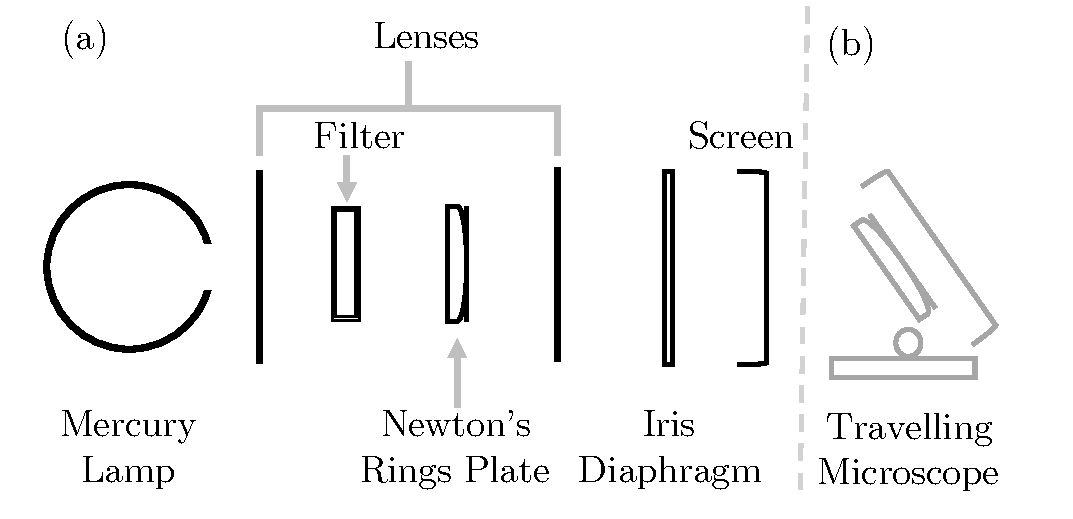
\includegraphics[width=5cm]{fig1}
\caption[]{A schematic of the experimental set-up used to collect data. }
\label{fig:fig1}
\end{center}
\end{figure}

An initial density of water was calculated by taking four measurements of the volume and mass of the water, then calculating four values for $\rho_{water}$, and then averaging it so find a value. 

One set of data was taken for each of the three capillary tubes that were used. Each tube varied in their internal diameter. These values were calculated from multiple measurements taken using a travelling microscope along the horizontal axis. The total length of the tube, from end to end, was measured using a ruler. 

The collected data was then applied to a least square fitting to create an initial linear model. The difference between the model and the data was then calculated, then this was divided by the uncertainty on the flow rate - this became our normalised residuals. Finally, these values were squared and summed up to a create a chi-squared value, then this was divided by the number of degrees of freedom to create the reduced chi-squared statistic. This analysis was performed to check if the model would hold true and if our data was accurate. After analysis three values of viscosity were calculated from the data. 

\vspace{-3ex}
\section{Results}
\vspace{-2ex}

The volumetric flow rate of water is plotted against the varying height, as shown in Fig. \ref{fig:fig2}. This flow rate was calculated by dividing each value of the measured volume with the measured time period. Using this data, a value of viscosity could be calculated through a rearranged form of equation [\ref{pohagen}],

\begin{equation} 
\eta=\frac{\pi \rho g a^4 }{8 L m}, 
\label{r-pohagen}
\end{equation}

where $m$ is the gradient of the least squares regression line, calculated with the known data for $dV/dt$ and $h$.

From preliminary results taking, our calculated value for the density of water, which was used in further calculations is $1001 \pm 1 kg m^{-1}$.

The calculated values for the viscosity of water are shown in Table \ref{table:1} with which respective tube was used, the radius, the reduced $\chi^2$, and the Durbin-Watson statistic ($\mathcal{D}$) for each of those tubes. 

An average value for viscosity can thus be found to be $1.00 \pm 0.03 mPa\cdot{s}$, which [does/does not?] agree with the literature value \cite{crc}, $1.31m \pm ?? Pa\cdot{s}$. 

\vspace{-1ex}
\begin{figure}[!h]
\begin{center}
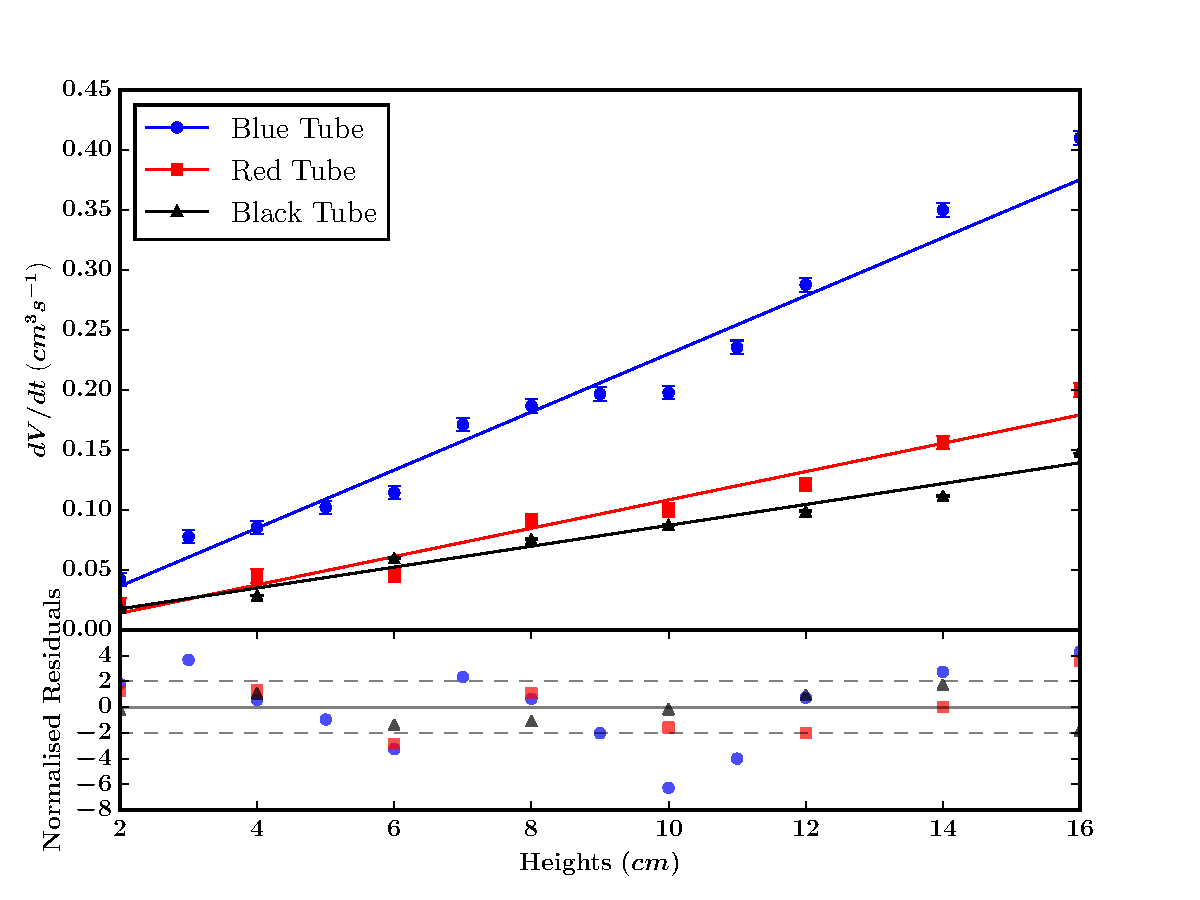
\includegraphics[width=9cm]{fig1-2}
\caption[]{The volume flow rate of water ($dV/dt$) as a function of height ($h$) for three capillary tubes of different diameter. The vertical error bars on $dV/dt$ are too small to be seen.}
\label{fig:fig2}
\end{center}
\end{figure}

\begin{table}[h!]
\centering
\begin{tabular}{ |c|c|c|c|c| } 
 \hline
 \textbf{Tube} & \textbf{Radius, a $[mm]$} & \textbf{$\boldsymbol{\eta_{water}}$ $[mPa\cdot{s}]$} & \textbf{$\boldsymbol{\chi^2_{\nu}}$} & $\mathcal{D}$\\ [0.5ex] 
 \hline\hline
 $Blue$ &$0.55\pm0.03$ & $1.0\pm0.2$ & 11.0 & 1.11\\ 
 $Red$ & $0.47\pm0.03$ & $1.1\pm0.3$ & 5.31 & 2.20\\
 $Black$ & $0.46\pm0.03$ & $1.0\pm0.3$ & 1.94 & 2.91\\
 
 \hline
\end{tabular}
\caption{Radius of the three tubes, their respective calculated value for $\eta_{water}$, the reduced chi-squared statistic, $\chi^2$, and the calculated Durbin-Watson statistic, $\mathcal{D}$, is shown for each tube as well.}
\label{table:1}
\end{table}


\vspace{-3ex}
\section{Discussion}
\vspace{-2ex}
From an initial inspection of Fig. \ref{fig:fig2} we see that the variation of $dV/dt$ with $h$ for the blue and red tubes do not appear to fit a linear regression model, while the black tube does appear to have a more linear trend. We can also see that the majority of the points and their respective error bars for all three sets of data do not seem to be within the lines of best fit. This implies that either our initial assumption of linearity in our data is not valid, or that there were some defects in the experiment. 

We can further explore the validity of our model by looking at the calculated values for $\chi^2_{\nu}$. A reasonable fit to the data should see $\chi^2_{\nu}$ to be approximately one \cite{hughesandhayes}. We find that for our data, the blue and red tubes $\chi^2_{\nu}$s  are not close to one at all, but with the black tube, while not exactly one, it is a similar value. This affirms our initial assumption that the data for the black tube has more linearity, while we should consider changing the theoretical model for the other two tubes. 

Experimentally, we can consider that there were some limitations with how the data was collected. For the volume of the water, it was likely that some water was left within the pipette thus causing some of the data for $V$ to be not its true value [[?!]]. This was also the case for when the capillary tube was attached, the rubber seal was not perfectly air tight so water did leak out, leading to similar problems. This can be potentially remedied by... However, with what time we had, we made do and ensured that no water was unaccounted for during the flowing part [[?]]

There was a systematic error in the LINEST model due to the values not being 0 and whatnot... 

Considerations of other factors were not taken into account such as the variation in the density of water with temperature change \cite{dentemp}. From the Thiesen-Scheel-Diesselhorst equation, we see that as the temperature of water increases, the density of water decreases, meaning that the viscosity of water will decrease as a result. [[too much usage of water]] 

The arising of random errors can not be considered as n

If further analysis is performed of the data we further see that there were problems with our chosen model. If we look at firstly the 

How can our experiment be limited? The volume - what changes the data, think of the setup  


% should this paragraph be in here so early?
However, from Table \ref{table:1} we see that $\eta_{water}$ for each tube are in agreement within their experimental errors. While the model may not be correct, the values produced, which when averaged [are/are not] in agreement with literature values. 

The temperature of the environment also varied, a value was recorded during each measurement. Enviroment temperature has an effect. 

The experiment was limited by difficulties in measurement, the amount of data unable to be taken - more data could have been taken to account for the temperature change maybe. Also repeat measurements so the mean and standard error could be used instead of trying to calculate values yourself. More time needed so more data, in the time given, only one set of data was taken for each tube so that different flow rates could be considered. 

We can also draw that for varying radii sizes, the values are consistent? 

\vspace{-5ex}
\section{Conclusions}
\vspace{-2ex}
 
In conclusion, through experimentation it is possible to calculate values for the viscosity of water which are similar to 

\begin{thebibliography}{5}
\bibitem{poiseuillehagen}
	Salvatore P. Sutera and Richard Skalak
	\textit{The History of Poiseuille's Law}.
	Annu. Rev. Fluid Mech., 1993.
	
\bibitem{collegephysics}
	Raymond A. Serway, Chris Vuille, and Jerry S. Faughin
	\textit{College Physics, 8th Edition}.
	Brooks/Cole, Belmont, CA, USA, 2009.

\bibitem{youngandfreedman} 
	Hugh D. Young and Roger A. Freedman.
	\textit{University Physics with Modern Physics, 13th Edition}. 
	Pearson Education Limited, Essex, UK, 2015.
	
\bibitem{crc} 
	David R. Lie
	\textit{CRC Handbook of Chemistry and Physics, 84th Edition}. 
	CRC Press, Florida, USA, 2004.
	
\bibitem{dentemp} 
	J. L. Martin and S. C. McCutcheon
	\textit{Hydrodynamics and Transport for Water Quality Modelling}. 
	CRC Press, Florida, USA, 1999.
	
\bibitem{hughesandhayes} 
	I. G. Hughes and T. P. A. Hase
	\textit{Measurements and their Uncertainties}. 
	Oxford University Press, Oxford, UK, 2010.
	
\end{thebibliography}
\clearpage

\vfill
\twocolumngrid
\vspace{-3ex}
\section*{Appendix}
\vspace{-2ex}

WIP

\clearpage
\end{document}